% !TeX spellcheck = en_US 
\documentclass[report]{byu-aero}

%This sets the visible levels shown on the Table of Contents. 2 will show the Sections and Subsections. This seems okay to save some space. If you want to show subsubsections change it to 3. 1 will just show the sections, but that seems too brief.
\setcounter{tocdepth}{2}

\usepackage{multirow}

%!!!!!!!!!!!!!!!!!!!!!!!!!!!!!!!!!!!!!!!!!!!!!!!!!!!!!!!!!!!!!!!!!!!!!!!!!!!!!!!!!!!!!!!!%
%!!!!!!! UNLESS YOU KNOW WHAT YOU'RE DOING, DO NOT TOUCH ANYTHING ABOVE THIS LINE !!!!!!!%
%!!!!!!!!!!!!!!!!!!!!!!!!!!!!!!!!!!!!!!!!!!!!!!!!!!!!!!!!!!!!!!!!!!!!!!!!!!!!!!!!!!!!!!!!%

%%%%%%%%%%%%%%%%%%%%%%%%%%%%%%%%%%
%%%%%%%%%%   Text Body   %%%%%%%%%
%%%%%%%%%%%%%%%%%%%%%%%%%%%%%%%%%%
\begin{document}

% Title Page

\includepdf[page=-]{titlepage.pdf}

%%%%%%%%%%%%%%%%%%%%%%%%%%%%%%%%%%%%%%%%%%
%%%%%%%%%%   Table of Contents   %%%%%%%%%
%%%%%%%%%%%%%%%%%%%%%%%%%%%%%%%%%%%%%%%%%%
\setcounter{page}{2} %This sets the page counter to 2, since the Title page is counted as page 1
\thispagestyle{tocpage} %This uses the alternate table of contents page header style
\tableofcontents %This makes the table of contents
%The following 3 lines add the Table of Contents "section" to the Table of Contents
%\phantomsection
%\addcontentsline{toc}{section}{Table of Contents}
%\markboth{Table of Contents}{Table of Contents}

\clearpage
\newpage

%%%%%%%%%%%%%%%%%%%%%%%%%%%%%%%%%%%%%%%%%%%%%%%%%%%%%%%%%%%%%%%%%%%%%%%%%%%%%%%%%%%%%%%%%
%%%%%%%%%%%%%%%%%%%%%%%%%%%%         EXECUTIVE SUMMARY         %%%%%%%%%%%%%%%%%%%%%%%%%%
%%%%%%%%%%%%%%%%%%%%%%%%%%%%%%%%%%%%%%%%%%%%%%%%%%%%%%%%%%%%%%%%%%%%%%%%%%%%%%%%%%%%%%%%%
\section{Executive Summary} % (5 Points)
\label{sec:ExecutiveSummary}
% Section Requirements
% 1) Maximum of 1 page. If exceeded, score as 0 points
% 2) Summary description of selected design and why it best meets the mission requirements
% 3) Main points from subsequent sections
% 4) Document the performance/capabilities of your system solution


% Performance Summary Table
\begin{table}[h!]
	\centering
	\caption{Summary of major system perfomance factors.}
	\label{tab:performancesummary}
	\rowcolors{2}{BYUbluelite}{white}
	\begin{tabular}{ |c|c| } 
		\hline
		\rowcolor{BYUbluemid}
    	Metric & \\ 
		\hline
	     & Performance (units) \\ 
		\hline
		 & Performance (units) \\ 
		\hline
	\end{tabular}
\end{table}

%%%%%%%%%%%%%%%%%%%%%%%%%%%%%%%%%%%%%%%%%%%%%%%%%%%%%%%%%%%%%%%%%%%%%%%%%%%%%%%%%%%%%%%%%
%%%%%%%%%%%%%%%%%%%%%%%%%%%%         MANAGEMENT SUMMARY        %%%%%%%%%%%%%%%%%%%%%%%%%%
%%%%%%%%%%%%%%%%%%%%%%%%%%%%%%%%%%%%%%%%%%%%%%%%%%%%%%%%%%%%%%%%%%%%%%%%%%%%%%%%%%%%%%%%%
\section{Management Summary} % (5 Points)
\label{sec:ManagementSummary}
% Section Requirements
% 1) Describe the organization of the design team
% 2) Chart of design personnel and assignments areas
% 3) Milestone chart showing planned and actual timing of major elements


%Team Organization Chart:
%TEAM ORGANIZATION
\begin{wrapfigure}[7]{R}{0in}
	\centering
	\raisebox{0pt}[\dimexpr\height-3\baselineskip\relax]{
\begin{tikzpicture}[node distance = 1cm, auto]

	% Place nodes
	\node [block] (Project Manager) {\footnotesize Project Manager};
%	\node [block, below left = 0.1 and -1.25cm  of Project Manager] (Engineering Lead) {\footnotesize Engineering Lead};
%	\node [block, below right = 0.1 and -1.25cm   of Project Manager] (Project Manager) {\footnotesize Project Manager};

	\node [block2, below left = 0.25 and -1.25cm of Project Manager] (Aerodynamics) {\footnotesize Aerodynamics};
	\node [block2, below left = 1.0 and -1.25cm  of Project Manager] (Structures) {\footnotesize Structures};
	\node [block2, below left = 1.75 and -1.25cm  of Project Manager] (Propulsion) {\footnotesize Propulsion};
	\node [block2, below right = 0.25 and -1.25cm  of Project Manager] (Systems) {\footnotesize Systems};
	\node [block2, below right = 1.0 and -1.25cm  of Project Manager] (Graphics) {\footnotesize Graphics};
	\node [block2, below right = 1.75 and -1.25cm  of Project Manager] (Manufacturing) {\footnotesize Manufacturing};

	% Draw edges
%	\path[line] let \p1=(Project Manager.south), \p2=(Engineering Lead.east) in (Project Manager.south) --  +(0,0.55*\y2) -| node {} (Engineering Lead.east);
%	\path[line] let \p1=(Project Manager.south), \p2=(Project Manager.west) in (Project Manager.south) -- +(0,0.55*\y2) -| node {} (Project Manager.west);

	\path[line] let \p1=(Project Manager.south), \p2=(Aerodynamics.east) in (Project Manager.south) -- +(0,0.65*\y2) -| node  {} (Aerodynamics.east);
	\path[line] let \p1=(Project Manager.south), \p2=(Systems.west) in (Project Manager.south) -- +(0,0.65*\y2) -| node  {} (Systems.west);

	\path[line] let \p1=(Project Manager.south), \p2=(Structures.east) in (Project Manager.south) -- +(0,0.8*\y2) -| node  {} (Structures.east);
	\path[line] let \p1=(Project Manager.south), \p2=(Graphics.west) in (Project Manager.south) -- +(0,0.8*\y2) -| node  {} (Graphics.west);

	\path[line] let \p1=(Project Manager.south), \p2=(Propulsion.east) in (Project Manager.south) -- +(0,0.85*\y2) -| node  {} (Propulsion.east);
	\path[line] let \p1=(Project Manager.south), \p2=(Manufacturing.west) in (Project Manager.south) -- +(0,0.85*\y2) -| node  {} (Manufacturing.west);
\end{tikzpicture}}
	\caption{Here we show the structure of, and assignment areas within, our team organization.}
	\label{fig:personnelassignments}
\end{wrapfigure} %You can change the team_organization.tex file to update this and it will automatically update in this file.


\begin{figure}[h!]
	\centering
	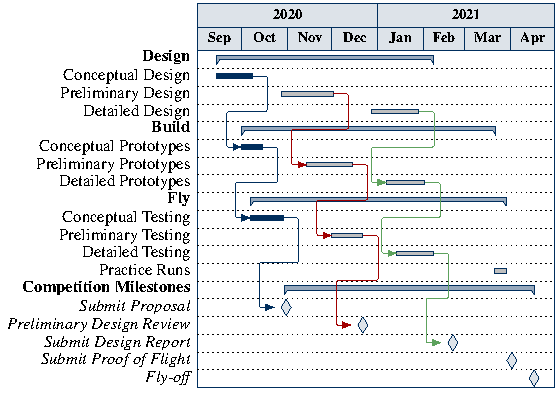
\includegraphics[width=4.5in]{ganttchart.pdf}
	\caption{This milestone chart reveals our {\color{\BYUblue} original plan} for major elements of our design process compared to the  {\color{\BYUred} actual timing} of these events.  Note that we submitted the proposal on time, as well as this report.  We anticipate remaining on schedule for the {\color{\BYUgreen} future elements} of this chart.}
	\label{fig:plannedvsactualtiming}
\end{figure}

%%%%%%%%%%%%%%%%%%%%%%%%%%%%%%%%%%%%%%%%%%%%%%%%%%%%%%%%%%%%%%%%%%%%%%%%%%%%%%%%%%%%%%%%%
%%%%%%%%%%%%%%%%%%%%%%%%%%%%         CONCEPTUAL DESIGN         %%%%%%%%%%%%%%%%%%%%%%%%%%
%%%%%%%%%%%%%%%%%%%%%%%%%%%%%%%%%%%%%%%%%%%%%%%%%%%%%%%%%%%%%%%%%%%%%%%%%%%%%%%%%%%%%%%%%
\section{Conceptual Design} % (15 Points) %Note: this should be completed already as part of the proposal
\label{sec:ConceptualDesign}
% Section Requirements
% 1) Describes mission requirements (problem statement)
% 2) Translate mission requirements into sub system design requirements
% 3) Present a scoring sensitivity analysis.
% 4) Review solution concepts/configurations considered
% 5) Describe concept weighting and selection process and results


\subsection{Mission Requirements}
\label{ssec:missionreqs}



\subsection{Sub-system Design Requirements}
\label{ssec:systemreqs}

\subsubsection{Aerodynamic Requirements}
\label{sssec:aeroreqs}


\subsubsection{Structural Requirements}
\label{sssec:structreqs}


\subsubsection{Propulsion Requirements}
\label{sssec:propreqs}


\subsubsection{Specialty Requirements} %change this to be specifically what it is (like bomb drop or whatever the specific mission is)
\label{sssec:specialreqs}



\subsection{Scoring Sensitivity Analysis}
\label{ssec:scoringsensitivity}



\subsection{Concept Weighting and Selection Process}
\label{ssec:selectionprocess}


%----------------
%---   Figure of Merit (i.e. the weights used in decision matrices)
%----------------
\begin{table}[h!]
	\centering
	\caption{Figures of Merit}
	\label{tab:fom}
	\rowcolors{2}{BYUbluelite}{white}
	\begin{tabular}{ |c|c| } 
		\hline
		\rowcolor{BYUbluemid}
		Factor & Scale (1-5) \\ 
		\hline
		Weight & 5 \\ 
		\hline
		Drag & 4 \\ 
		\hline
		Simplicity & 3 \\ 
		\hline
		Stability & 2 \\ 
		\hline
		{\color{\BYUred} {\color{BYUred} [YEAR SPECIFIC ITEM]}} & 1 \\ 
		\hline
	\end{tabular}
\end{table}



%----------------
%---   Wing Configuration Decision Matrix (Convetional, Bi-Plane, Tandem Wing, etc.)
%----------------
\begin{table}[h!]
	\centering
	\caption{Weighted decision matrix for wing configuration.}
	\label{tab:wingconfiguration}
	\rowcolors{2}{BYUbluelite}{white}
	\begin{tabular}{ |c|c|c|c|c| } 
		\hline
		\rowcolor{BYUbluemid}
    	& & {\color{BYUred} [OPTION]} & {\color{BYUred} [OPTION]} & {\color{BYUred} [OPTION]} \\ 
		\rowcolor{BYUbluemid}
		\multirow{-2}{*}{Factor} & \multirow{-2}{*}{Scale}  & \parbox[c]{1in}{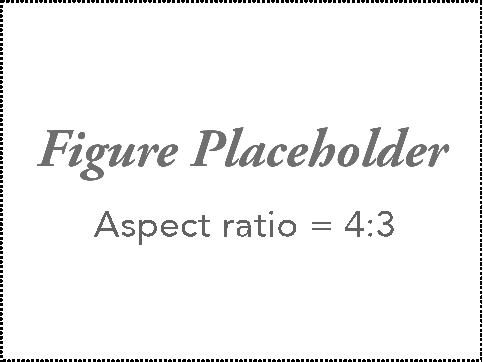
\includegraphics[width=1in]{draft4x3}} & \parbox[c]{1in}{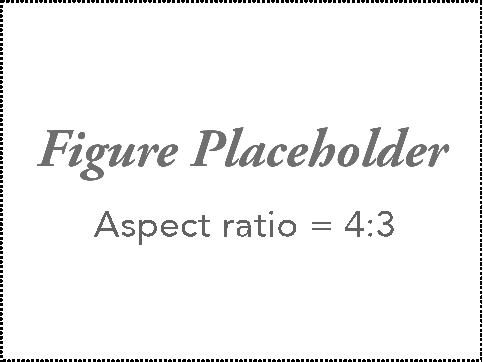
\includegraphics[width=1in]{draft4x3}} &  \parbox[c]{1in}{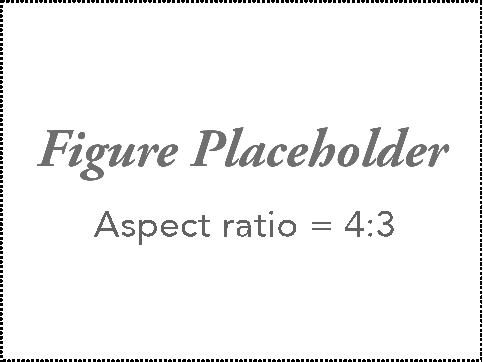
\includegraphics[width=1in]{draft4x3}} \\ 
		\hline
		Weight & 5 & & &\\ 
		\hline
		Drag & 4 & & & \\ 
		\hline
		Simplicity & 3 & & & \\ 
		\hline
		Stability & 2 & & & \\ 
		\hline
		{\color{\BYUred} {\color{BYUred} [YEAR SPECIFIC ITEM]}} & 1 & & & \\ 
		\hline
		\multicolumn{2}{|c|}{Totals} &  &  &  \\ %BOLD WINNING OPTION
		\hline
	\end{tabular}
\end{table}


%----------------
%---   Wing Placement Decision Matrix  (High, Mid, Low)
%----------------
\begin{table}[h!]
	\centering
	\caption{Weighted decision matrix for wing placement.}
	\label{tab:wingplacement}
	\rowcolors{2}{BYUbluelite}{white}
	\begin{tabular}{ |c|c|c|c|c| } 
		\hline
		\rowcolor{BYUbluemid}
		& & {\color{BYUred} [OPTION]} & {\color{BYUred} [OPTION]} & {\color{BYUred} [OPTION]} \\ 
		\rowcolor{BYUbluemid}
		\multirow{-2}{*}{Factor} & \multirow{-2}{*}{Scale}  & \parbox[c]{1in}{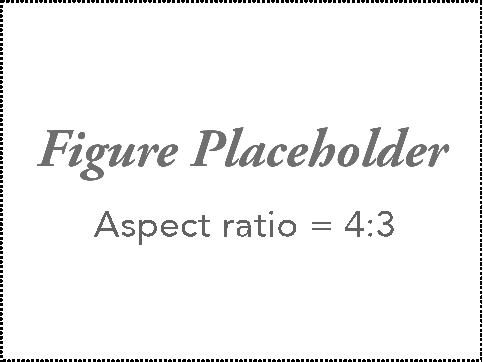
\includegraphics[width=1in]{draft4x3}} & \parbox[c]{1in}{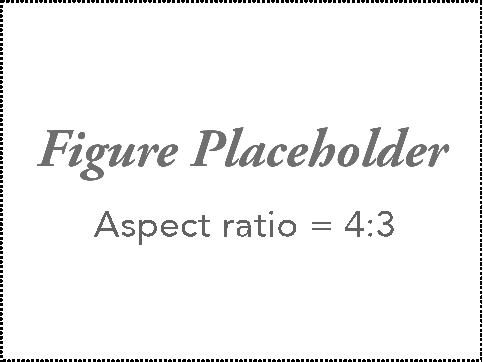
\includegraphics[width=1in]{draft4x3}} &  \parbox[c]{1in}{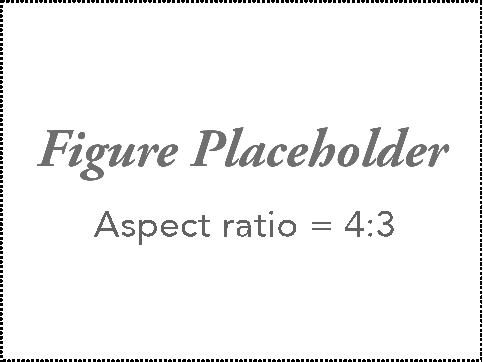
\includegraphics[width=1in]{draft4x3}} \\ 
		\hline
		Weight & 5 & & &\\ 
		\hline
		Drag & 4 & & & \\ 
		\hline
		Simplicity & 3 & & & \\ 
		\hline
		Stability & 2 & & & \\ 
		\hline
		{\color{\BYUred} {\color{BYUred} [YEAR SPECIFIC ITEM]}} & 1 & & & \\ 
		\hline
		\multicolumn{2}{|c|}{Totals} &  &  &  \\ %BOLD WINNING OPTION
		\hline
	\end{tabular}
\end{table}


%----------------
%---  Tail Configuration Decision Matrix  (Conventional, H-tail, V-tail, Flying wing, etc.)
%----------------
\begin{table}[h!]
	\centering
	\caption{Weighted decision matrix for tail configuration.}
	\label{tab:tailconfiguration}
	\rowcolors{2}{BYUbluelite}{white}
	\begin{tabular}{ |c|c|c|c|c| } 
		\hline
		\rowcolor{BYUbluemid}
		& & {\color{BYUred} [OPTION]} & {\color{BYUred} [OPTION]} & {\color{BYUred} [OPTION]} \\ 
		\rowcolor{BYUbluemid}
		\multirow{-2}{*}{Factor} & \multirow{-2}{*}{Scale}  & \parbox[c]{1in}{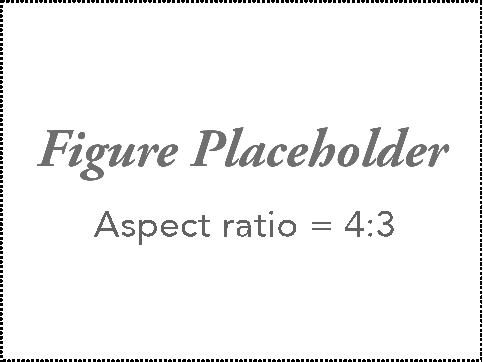
\includegraphics[width=1in]{draft4x3}} & \parbox[c]{1in}{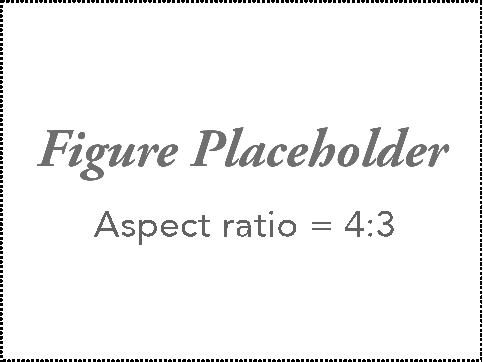
\includegraphics[width=1in]{draft4x3}} &  \parbox[c]{1in}{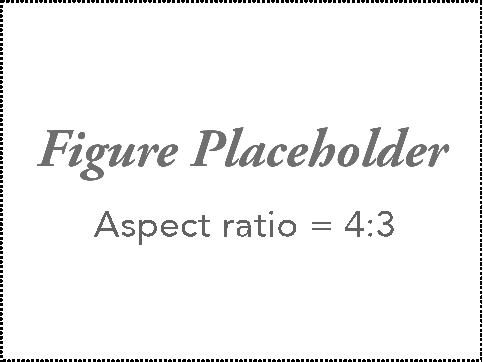
\includegraphics[width=1in]{draft4x3}} \\ 
		\hline
		Weight & 5 & & &\\ 
		\hline
		Drag & 4 & & & \\ 
		\hline
		Simplicity & 3 & & & \\ 
		\hline
		Stability & 2 & & & \\ 
		\hline
		{\color{\BYUred} {\color{BYUred} [YEAR SPECIFIC ITEM]}} & 1 & & & \\ 
		\hline
		\multicolumn{2}{|c|}{Totals} &  &  &  \\ %BOLD WINNING OPTION
		\hline
	\end{tabular}
\end{table}


%----------------
%---   Propulsion Configuration Decision Matrix  (single prop, dual prop, distributed propulsion, etc.)
%----------------
\begin{table}[h!]
	\centering
	\caption{Weighted decision matrix for propulsion configuration.}
	\label{tab:propconfiguration}
	\rowcolors{2}{BYUbluelite}{white}
	\begin{tabular}{ |c|c|c|c|c| } 
		\hline
		\rowcolor{BYUbluemid}
		& & {\color{BYUred} [OPTION]} & {\color{BYUred} [OPTION]} & {\color{BYUred} [OPTION]} \\ 
		\rowcolor{BYUbluemid}
		\multirow{-2}{*}{Factor} & \multirow{-2}{*}{Scale}  & \parbox[c]{1in}{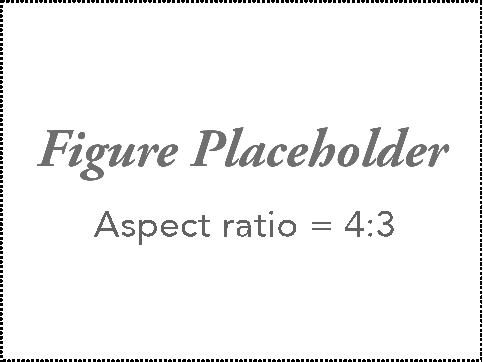
\includegraphics[width=1in]{draft4x3}} & \parbox[c]{1in}{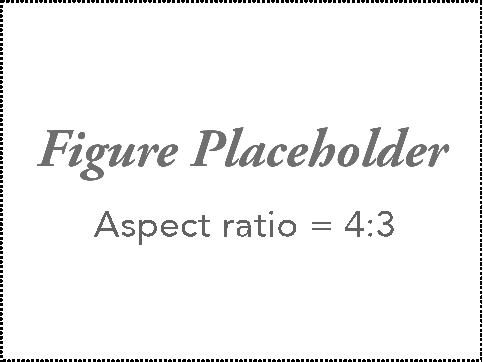
\includegraphics[width=1in]{draft4x3}} &  \parbox[c]{1in}{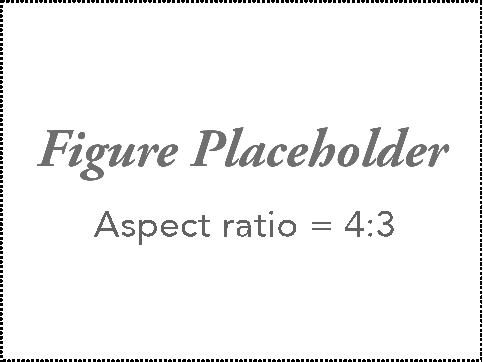
\includegraphics[width=1in]{draft4x3}} \\ 
		\hline
		Weight & 5 & & &\\ 
		\hline
		Drag & 4 & & & \\ 
		\hline
		Simplicity & 3 & & & \\ 
		\hline
		Stability & 2 & & & \\ 
		\hline
		{\color{\BYUred} {\color{BYUred} [YEAR SPECIFIC ITEM]}} & 1 & & & \\ 
		\hline
		\multicolumn{2}{|c|}{Totals} &  &  &  \\ %BOLD WINNING OPTION
		\hline
	\end{tabular}
\end{table}



%----------------
%---   Propulsion Placement Decision Matrix  (tractor, pusher, etc)
%----------------
\begin{table}[h!]
	\centering
	\caption{Weighted decision matrix for wing placement.}
	\label{tab:propplacement}
	\rowcolors{2}{BYUbluelite}{white}
	\begin{tabular}{ |c|c|c|c|c| } 
		\hline
		\rowcolor{BYUbluemid}
		& & {\color{BYUred} [OPTION]} & {\color{BYUred} [OPTION]} & {\color{BYUred} [OPTION]} \\ 
		\rowcolor{BYUbluemid}
		\multirow{-2}{*}{Factor} & \multirow{-2}{*}{Scale}  & \parbox[c]{1in}{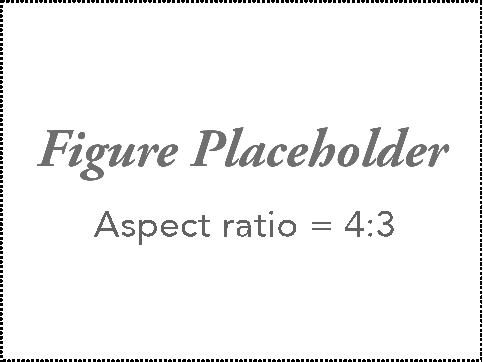
\includegraphics[width=1in]{draft4x3}} & \parbox[c]{1in}{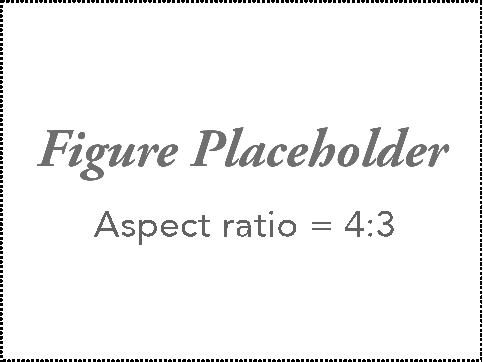
\includegraphics[width=1in]{draft4x3}} &  \parbox[c]{1in}{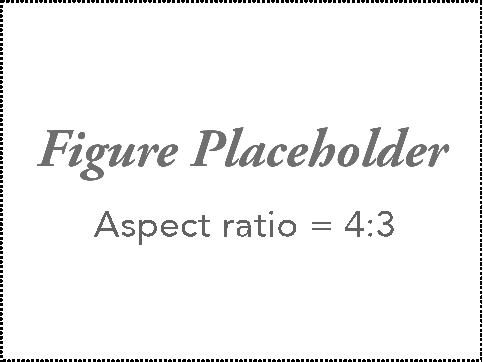
\includegraphics[width=1in]{draft4x3}} \\ 
		\hline
		Weight & 5 & & &\\ 
		\hline
		Drag & 4 & & & \\ 
		\hline
		Simplicity & 3 & & & \\ 
		\hline
		Stability & 2 & & & \\ 
		\hline
		{\color{\BYUred} {\color{BYUred} [YEAR SPECIFIC ITEM]}} & 1 & & & \\ 
		\hline
		\multicolumn{2}{|c|}{Totals} &  &  &  \\ %BOLD WINNING OPTION
		\hline
	\end{tabular}
\end{table}



%----------------
%---   Payload Decision Matrix.
%----------------
\begin{table}[h!]
	\centering
	\caption{Weighted decision matrix for {\color{\BYUred} [SPECIFY THIS YEAR'S PAYLOAD DESIGN]}.}
	\label{tab:payloadconfiguration}
	\rowcolors{2}{BYUbluelite}{white}
	\begin{tabular}{ |c|c|c|c|c| } 
		\hline
		\rowcolor{BYUbluemid}
		& & {\color{BYUred} [OPTION]} & {\color{BYUred} [OPTION]} & {\color{BYUred} [OPTION]} \\ 
		\rowcolor{BYUbluemid}
		\multirow{-2}{*}{Factor} & \multirow{-2}{*}{Scale}  & \parbox[c]{1in}{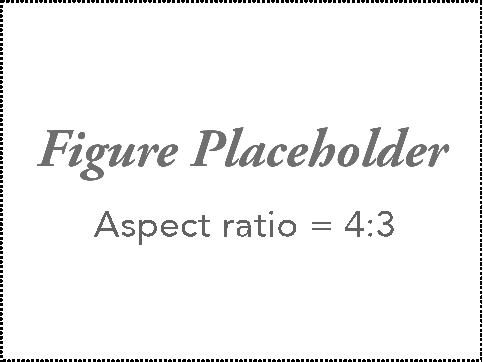
\includegraphics[width=1in]{draft4x3}} & \parbox[c]{1in}{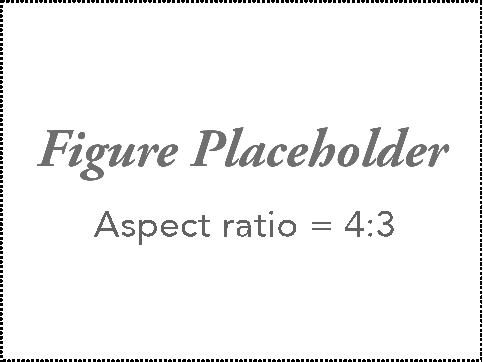
\includegraphics[width=1in]{draft4x3}} &  \parbox[c]{1in}{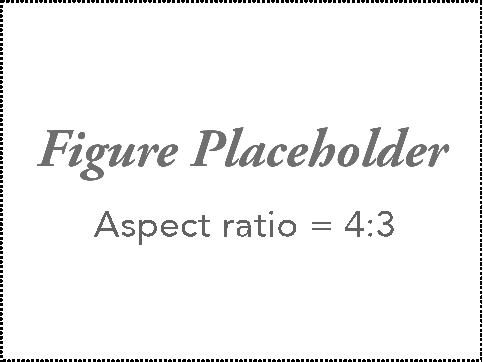
\includegraphics[width=1in]{draft4x3}} \\ 
		\hline
		Weight & 5 & & &\\ 
		\hline
		Drag & 4 & & & \\ 
		\hline
		Simplicity & 3 & & & \\ 
		\hline
		Stability & 2 & & & \\ 
		\hline
		{\color{\BYUred} {\color{BYUred} [YEAR SPECIFIC ITEM]}} & 1 & & & \\ 
		\hline
		\multicolumn{2}{|c|}{Totals} &  &  &  \\ %BOLD WINNING OPTION
		\hline
	\end{tabular}
\end{table}



\subsubsection{Final Concept}
\label{sssec:finalconcept}

%----------------
%---  Figure of the final concept
%----------------
\begin{figure}[h!]
	\centering
	
\includegraphics[width=3.5in]{draft.pdf}
	\caption{Our final conceptual design incorporates the highest scoring options in the decision matrices described above.}
	\label{fig:finalconcept}
\end{figure}



%%%%%%%%%%%%%%%%%%%%%%%%%%%%%%%%%%%%%%%%%%%%%%%%%%%%%%%%%%%%%%%%%%%%%%%%%%%%%%%%%%%%%%%%%
%%%%%%%%%%%%%%%%%%%%%%%%%%%%         PRELIMINARY DESIGN        %%%%%%%%%%%%%%%%%%%%%%%%%%
%%%%%%%%%%%%%%%%%%%%%%%%%%%%%%%%%%%%%%%%%%%%%%%%%%%%%%%%%%%%%%%%%%%%%%%%%%%%%%%%%%%%%%%%%
\section{Preliminary Design} % (20 Points)
\label{sec:PreliminaryDesign}
% Section Requirements
% 1) Describe design/analysis methodology
% 2) Document design/sizing trades
% 3) Describe/document methodology for prediction of aircraft performance (include capabilities and uncertainties)
% 4) Provide estimates of the aircraft lift, drag and stability characteristics and method of prediction
% 5) Provide estimates of the aircraft mission performance 


\subsection{Methodology}
\label{ssec:methodology}




\subsection{Trade Studies}
\label{ssec:tradestudies}




\subsection{Estimated Aircraft Performance}
\label{ssec:estaircraftperfomance}




\subsubsection{Performance Prediction Methodologies and Uncertainties}
\label{sssec:uncertaintyanalysis}




\subsubsection{Lift and Drag}
\label{sssec:liftdrag}




\subsubsection{Stability}
\label{sssec:stability}



\subsubsection{Mission Performance}
\label{sssec:missionperformance}





%%%%%%%%%%%%%%%%%%%%%%%%%%%%%%%%%%%%%%%%%%%%%%%%%%%%%%%%%%%%%%%%%%%%%%%%%%%%%%%%%%%%%%%%%
%%%%%%%%%%%%%%%%%%%%%%%%%%%%           DETAIL DESIGN           %%%%%%%%%%%%%%%%%%%%%%%%%%
%%%%%%%%%%%%%%%%%%%%%%%%%%%%%%%%%%%%%%%%%%%%%%%%%%%%%%%%%%%%%%%%%%%%%%%%%%%%%%%%%%%%%%%%%
\section{Detail Design} % (15 Points + 15 Points for Drawing Package)
\label{sec:detaildesign}
% Section Requirements
% 1) Document dimensional parameters of final design
% 2) Document structural characteristics/capabilities of final design
% 3) Document systems and sub-systems selection/integration/architecture
% 4) Document Weight and Balance for final design
% 5) Must include Weight \& Balance table empty and with each possible payload/configuration
% 6) Document flight performance parameters for final design
% 7) Document mission performance for final design




\subsection{Sizing}
\label{ssec:sizing}




\subsection{Structures}
\label{ssec:structures}




\subsection{System Selection, Integration, and Architecture}
\label{ssec:systemdetails}




\subsection{Weights and Balance}
\label{ssec:weightsandbalance}


%----------------
%---  Weight and Balance Table
%----------------
\begin{table}[h!]
	\centering
	\caption{Weight and Balance table including empty aircraft and each possible configuration.}
	\label{tab:wieghtsandbalance}
	\rowcolors{2}{BYUbluelite}{white}
	\begin{tabular}{ |c|c|c| } 
		\hline
		\rowcolor{BYUbluemid}
    	Configuration & Weight (grams) & CG Location (mm) \\ 
		\hline
	    Mission 1 &  &  \\ 
		\hline
		Mission 2 &  &  \\ 
		\hline
		Mission 3 &  &  \\ 
		\hline
	\end{tabular}
\end{table}



\subsection{Flight Performance Parameters}
\label{ssec:flightperformanceparams}




\subsection{Mission Performance}
\label{ssec:missionperformance}



 
\subsection{Drawing Package}
\label{ssec:drawings}

The following are drawings including a 3-View drawing with dimensions of all configurations, a structural arrangement drawing, a systems layout/location drawing, and payload accommodation drawings.

%%%%%%%%%%%%%%%%%%%%%%%%%%%%%%%%%%%%%%%%%%%%%%
%%%%%%%%%%%%%   DRAWING PACKAGE   %%%%%%%%%%%%
%%%%%%%%%%%%%%%%%%%%%%%%%%%%%%%%%%%%%%%%%%%%%%
% Drawing package Requirements:
% 1) 3-View drawing with dimensions of all configurations
% 2) Structural arrangement drawing
% 3) Systems layout/location drawing
% 4) Payload(s) accommodation drawing(s)


%----------------
% 3-view drawing

\includepdf[page=-]{draft.pdf}
%----------------
% Structural Arrangement Drawing

\includepdf[page=-]{draft.pdf}
%----------------
% Systems Layout/Location Drawing

\includepdf[page=-]{draft.pdf}
%----------------
% Payload Accommodation drawing

\includepdf[page=-]{draft.pdf}
%----------------


%%%%%%%%%%%%%%%%%%%%%%%%%%%%%%%%%%%%%%%%%%%%%%%%%%%%%%%%%%%%%%%%%%%%%%%%%%%%%%%%%%%%%%%%%
%%%%%%%%%%%%%%%%%%%%%%%%%%          MANUFACTURING PLAN          %%%%%%%%%%%%%%%%%%%%%%%%%
%%%%%%%%%%%%%%%%%%%%%%%%%%%%%%%%%%%%%%%%%%%%%%%%%%%%%%%%%%%%%%%%%%%%%%%%%%%%%%%%%%%%%%%%%
\section{Manufacturing Plan} % (5 Points)
\label{sec:ManufacturingPlan}
% Section Requirements
% 1) Document the process selected for major component manufacture
% 2) Manufacturing processes investigated and selection process and results
% 3) Manufacturing milestones chart: plan and actual

%----------------
%---  Figure of Merit (i.e. the weights used in decision matrices)
%----------------
\begin{table}[h!]
	\centering
	\caption{Figures of Merit}
	\label{tab:fomman}
	\rowcolors{2}{BYUbluelite}{white}
	\begin{tabular}{ |c|c| } 
		\hline
		\rowcolor{BYUbluemid}
    	Factor & Relative Importance (1-5) \\ 
		\hline
	     &  \\ 
		\hline
		 &  \\ 
		\hline
		 &  \\ 
		\hline
		 &  \\ 
		\hline
		 &  \\ 
		\hline
	\end{tabular}
\end{table}


%----------------
%---   Wing Manufacture Decision Matrix  (single prop, dual prop, distributed propulsion, etc.)
%----------------
\begin{table}[h!]
	\centering
	\caption{Weighted decision matrix for wing manufacturing technique.}
	\label{tab:wingmanufacturedecision}
	\rowcolors{2}{BYUbluelite}{white}
	\begin{tabular}{ |c|c|c|c|c| } 
		\hline
		\rowcolor{BYUbluemid}
		& & {\color{BYUred} [OPTION]} & {\color{BYUred} [OPTION]} & {\color{BYUred} [OPTION]} \\ 
		\rowcolor{BYUbluemid}
		\multirow{-2}{*}{Factor} & \multirow{-2}{*}{Scale}  & \parbox[c]{1in}{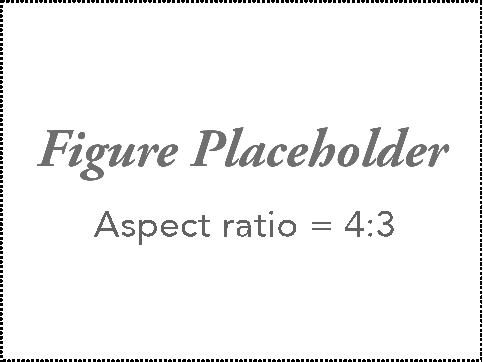
\includegraphics[width=1in]{draft4x3}} & \parbox[c]{1in}{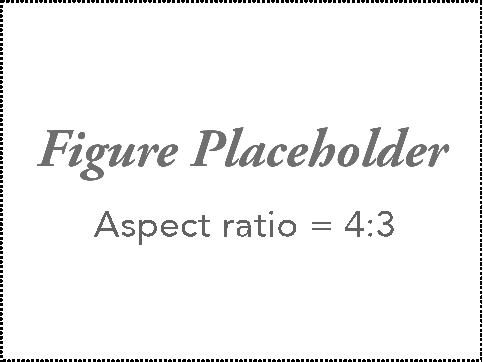
\includegraphics[width=1in]{draft4x3}} &  \parbox[c]{1in}{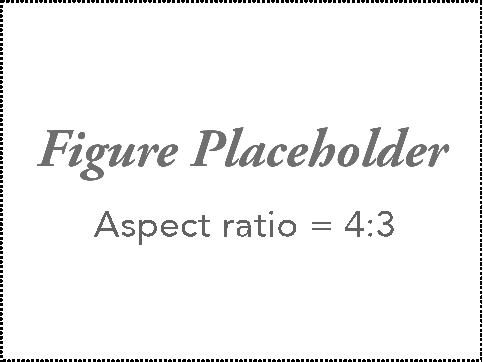
\includegraphics[width=1in]{draft4x3}} \\ 
		\hline
		Weight & 5 & & &\\ 
		\hline
		Drag & 4 & & & \\ 
		\hline
		Simplicity & 3 & & & \\ 
		\hline
		Stability & 2 & & & \\ 
		\hline
		{\color{\BYUred} {\color{BYUred} [YEAR SPECIFIC ITEM]}} & 1 & & & \\ 
		\hline
		\multicolumn{2}{|c|}{Totals} &  &  &  \\ %BOLD WINNING OPTION
		\hline
	\end{tabular}
\end{table}



%----------------
%---   Fuselage Manufacture Decision Matrix  (single prop, dual prop, distributed propulsion, etc.)
%----------------
\begin{table}[h!]
	\centering
	\caption{Weighted decision matrix for fuselage manufacturing technique.}
	\label{tab:fuselagemanufacturingdecision}
	\rowcolors{2}{BYUbluelite}{white}
	\begin{tabular}{ |c|c|c|c|c| } 
		\hline
		\rowcolor{BYUbluemid}
		& & {\color{BYUred} [OPTION]} & {\color{BYUred} [OPTION]} & {\color{BYUred} [OPTION]} \\ 
		\rowcolor{BYUbluemid}
		\multirow{-2}{*}{Factor} & \multirow{-2}{*}{Scale}  & \parbox[c]{1in}{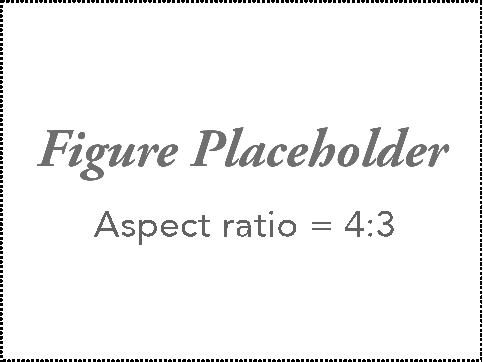
\includegraphics[width=1in]{draft4x3}} & \parbox[c]{1in}{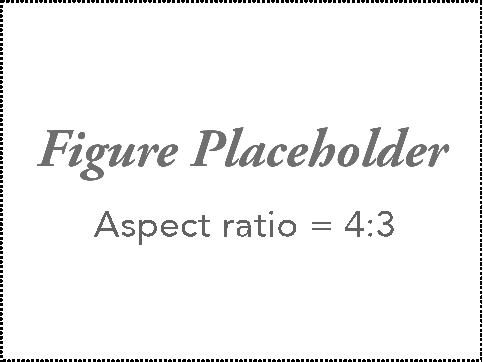
\includegraphics[width=1in]{draft4x3}} &  \parbox[c]{1in}{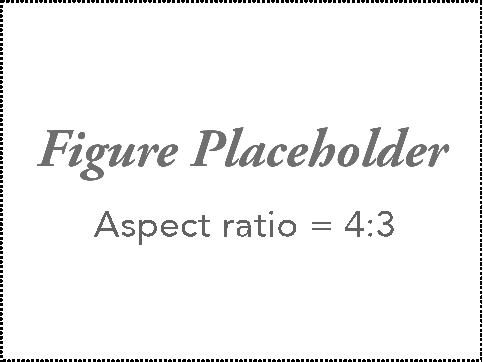
\includegraphics[width=1in]{draft4x3}} \\ 
		\hline
		Weight & 5 & & &\\ 
		\hline
		Drag & 4 & & & \\ 
		\hline
		Simplicity & 3 & & & \\ 
		\hline
		Stability & 2 & & & \\ 
		\hline
		{\color{\BYUred} {\color{BYUred} [YEAR SPECIFIC ITEM]}} & 1 & & & \\ 
		\hline
		\multicolumn{2}{|c|}{Totals} &  &  &  \\ %BOLD WINNING OPTION
		\hline
	\end{tabular}
\end{table}



%----------------
%---   Tail Manufacture Decision Matrix  (single prop, dual prop, distributed propulsion, etc.)
%----------------
\begin{table}[h!]
	\centering
	\caption{Weighted decision matrix for tail manufacturing technique.}
	\label{tab:tailmanufacturedecision}
	\rowcolors{2}{BYUbluelite}{white}
	\begin{tabular}{ |c|c|c|c|c| } 
		\hline
		\rowcolor{BYUbluemid}
		& & {\color{BYUred} [OPTION]} & {\color{BYUred} [OPTION]} & {\color{BYUred} [OPTION]} \\ 
		\rowcolor{BYUbluemid}
		\multirow{-2}{*}{Factor} & \multirow{-2}{*}{Scale}  & \parbox[c]{1in}{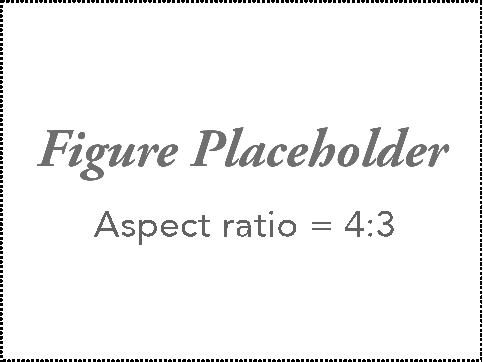
\includegraphics[width=1in]{draft4x3}} & \parbox[c]{1in}{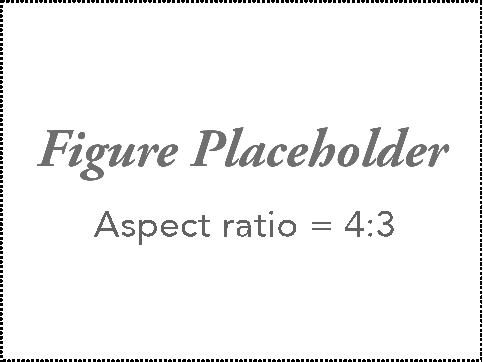
\includegraphics[width=1in]{draft4x3}} &  \parbox[c]{1in}{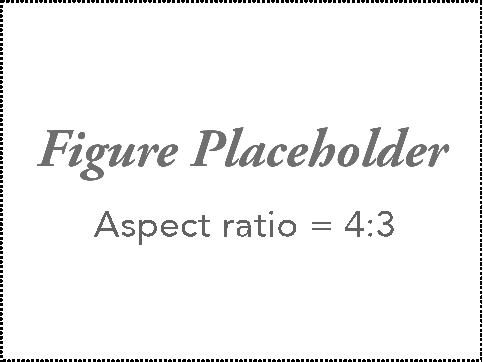
\includegraphics[width=1in]{draft4x3}} \\ 
		\hline
		Weight & 5 & & &\\ 
		\hline
		Drag & 4 & & & \\ 
		\hline
		Simplicity & 3 & & & \\ 
		\hline
		Stability & 2 & & & \\ 
		\hline
		{\color{\BYUred} {\color{BYUred} [YEAR SPECIFIC ITEM]}} & 1 & & & \\ 
		\hline
		\multicolumn{2}{|c|}{Totals} &  &  &  \\ %BOLD WINNING OPTION
		\hline
	\end{tabular}
\end{table}





%----------------
%---   Payload Manufacture Decision Matrix  (single prop, dual prop, distributed propulsion, etc.)
%----------------
\begin{table}[h!]
	\centering
	\caption{Weighted decision matrix for {\color{\BYUred} [SPECIFY THIS YEAR'S PAYLOAD DESIGN]}.}
	\label{tab:payloadmanufacturedecision}
	\rowcolors{2}{BYUbluelite}{white}
	\begin{tabular}{ |c|c|c|c|c| } 
		\hline
		\rowcolor{BYUbluemid}
		& & {\color{BYUred} [OPTION]} & {\color{BYUred} [OPTION]} & {\color{BYUred} [OPTION]} \\ 
		\rowcolor{BYUbluemid}
		\multirow{-2}{*}{Factor} & \multirow{-2}{*}{Scale}  & \parbox[c]{1in}{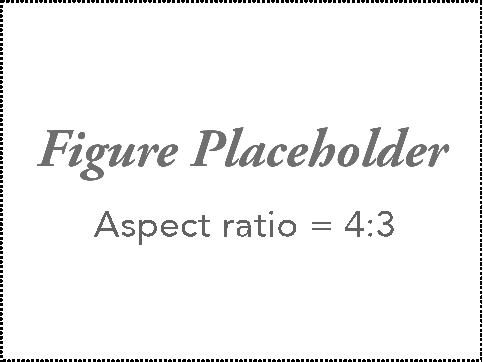
\includegraphics[width=1in]{draft4x3}} & \parbox[c]{1in}{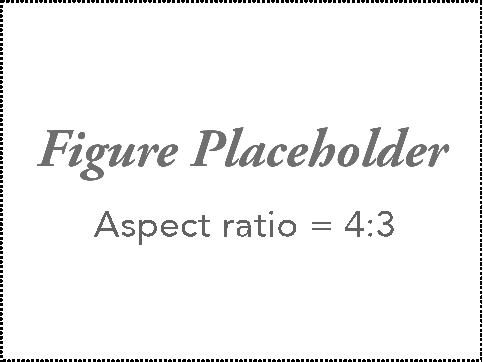
\includegraphics[width=1in]{draft4x3}} &  \parbox[c]{1in}{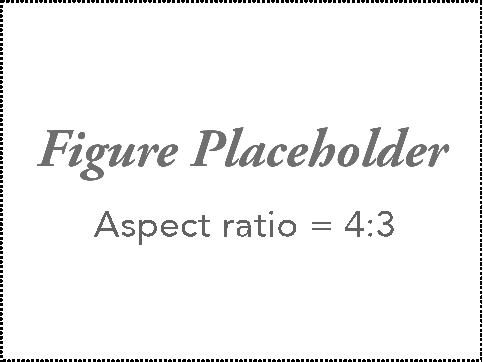
\includegraphics[width=1in]{draft4x3}} \\ 
		\hline
		Weight & 5 & & &\\ 
		\hline
		Drag & 4 & & & \\ 
		\hline
		Simplicity & 3 & & & \\ 
		\hline
		Stability & 2 & & & \\ 
		\hline
		{\color{\BYUred} {\color{BYUred} [YEAR SPECIFIC ITEM]}} & 1 & & & \\ 
		\hline
		\multicolumn{2}{|c|}{Totals} &  &  &  \\ %BOLD WINNING OPTION
		\hline
	\end{tabular}
\end{table}

%----------------
% ---  Manufacturing Milestone chart
%----------------
\begin{figure}[h!]
	\centering
	
\includegraphics[width=3.5in]{draft.pdf}
	\caption{This milestone chart reveals our original plan for major elements of our manufacturing process compared to the actual timing of these events.}
	\label{fig:plannedvsactualtimingmanufacturing}
\end{figure}



%%%%%%%%%%%%%%%%%%%%%%%%%%%%%%%%%%%%%%%%%%%%%%%%%%%%%%%%%%%%%%%%%%%%%%%%%%%%%%%%%%%%%%%%%
%%%%%%%%%%%%%%%%%%%%%%%%%%%%           TESTING PLAN            %%%%%%%%%%%%%%%%%%%%%%%%%%
%%%%%%%%%%%%%%%%%%%%%%%%%%%%%%%%%%%%%%%%%%%%%%%%%%%%%%%%%%%%%%%%%%%%%%%%%%%%%%%%%%%%%%%%%
\section{Testing Plan} % (5 points)
\label{sec:TestingPlan}
% Section Requirements
% 1) Describe all major ground and flight tests performed.
% 2) Objectives and schedule for each.
% 3) Data to be collected and how applied.
% 4) Test and flight check lists


\subsection{Completed Testing}
\label{ssec:completedtesting}




\subsubsection{Ground Testing}
\label{sssec:groundtesting}



\subsubsection{Flight Testing}
\label{sssec:flighttesting}



\subsection{Planned Testing}
\label{ssec:plannedtesting}



\subsection{Test and Flight Checklists}



%%%%%%%%%%%%%%%%%%%%%%%%%%%%%%%%%%%%%%%%%%%%%%%%%%%%%%%%%%%%%%%%%%%%%%%%%%%%%%%%%%%%%%%%%
%%%%%%%%%%%%%%%%%%%%%%%%%%          PERFORMANCE RESULTS          %%%%%%%%%%%%%%%%%%%%%%%%
%%%%%%%%%%%%%%%%%%%%%%%%%%%%%%%%%%%%%%%%%%%%%%%%%%%%%%%%%%%%%%%%%%%%%%%%%%%%%%%%%%%%%%%%%
\section{Performance Results} % (10 Points)
\label{sec:PerformanceResults}
% Section Requirements
% ) Describe the demonstrated performance of key subsystems following execution of testing plan
% ) Compare to predictions and explain any differences and improvements made
% ) Describe the demonstrated performance of your complete aircraft solution
% ) Compare to predictions and explain any differences and improvements made






%%%%%%%%%%%%%%%%%%%%%%%%%%%%%%%%%%%%%%%%%%%%%%%%%%%%%%%%%%%%%%%%%%%%%%%%%%%%%%%%%%%%%%%%%
%%%%%%%%%%%%%%%%%%%%%%%%%%%%           BIBLIOGRAPHY            %%%%%%%%%%%%%%%%%%%%%%%%%%
%%%%%%%%%%%%%%%%%%%%%%%%%%%%%%%%%%%%%%%%%%%%%%%%%%%%%%%%%%%%%%%%%%%%%%%%%%%%%%%%%%%%%%%%%
%Bibliography (5 Points)
% 1) List of all published works referenced in the text must be present in this section.
% 2) Any material taken from a published source in all previous sections must have a numerical subscript corresponding to the appropriate citation in this section.
% 3) References should appear in numerical order.
% 4) Format should match AIAA provided guidelines:
%\newpage
%\clearpage
\bibliography{ref}{}
\bibliographystyle{aiaa}

\end{document}